\documentclass[tikz,border=10pt]{standalone}
\usepackage{tikz}
\usetikzlibrary{arrows.meta,positioning,calc,backgrounds,fit,shapes.geometric}
\usepackage[scaled=0.92]{helvet}
\renewcommand{\familydefault}{\sfdefault}
\usepackage{amsmath,amssymb}
\definecolor{ink}{HTML}{262624}
\definecolor{mute}{HTML}{8A8984}
\definecolor{line}{HTML}{BDBBB5}
\definecolor{acc}{HTML}{2A78D6}
\definecolor{accbg}{HTML}{F1F6FD}
\tikzset{
  >={Latex[length=2.2mm]},
  every node/.style={text=ink},
  b/.style={draw=line, fill=white, rounded corners=2pt, align=center, inner sep=6pt,
            minimum height=10mm, text width=#1, font=\small},
  b/.default=40mm,
  a/.style={b=#1, draw=acc, fill=accbg},
  a/.default=40mm,
  t/.style={font=\footnotesize, text=mute, align=center},
  e/.style={->, draw=mute, line width=0.6pt},
  ea/.style={->, draw=acc, line width=0.9pt},
  eh/.style={->, draw=acc, line width=0.9pt, dash pattern=on 3pt off 2pt},
}

\begin{document}
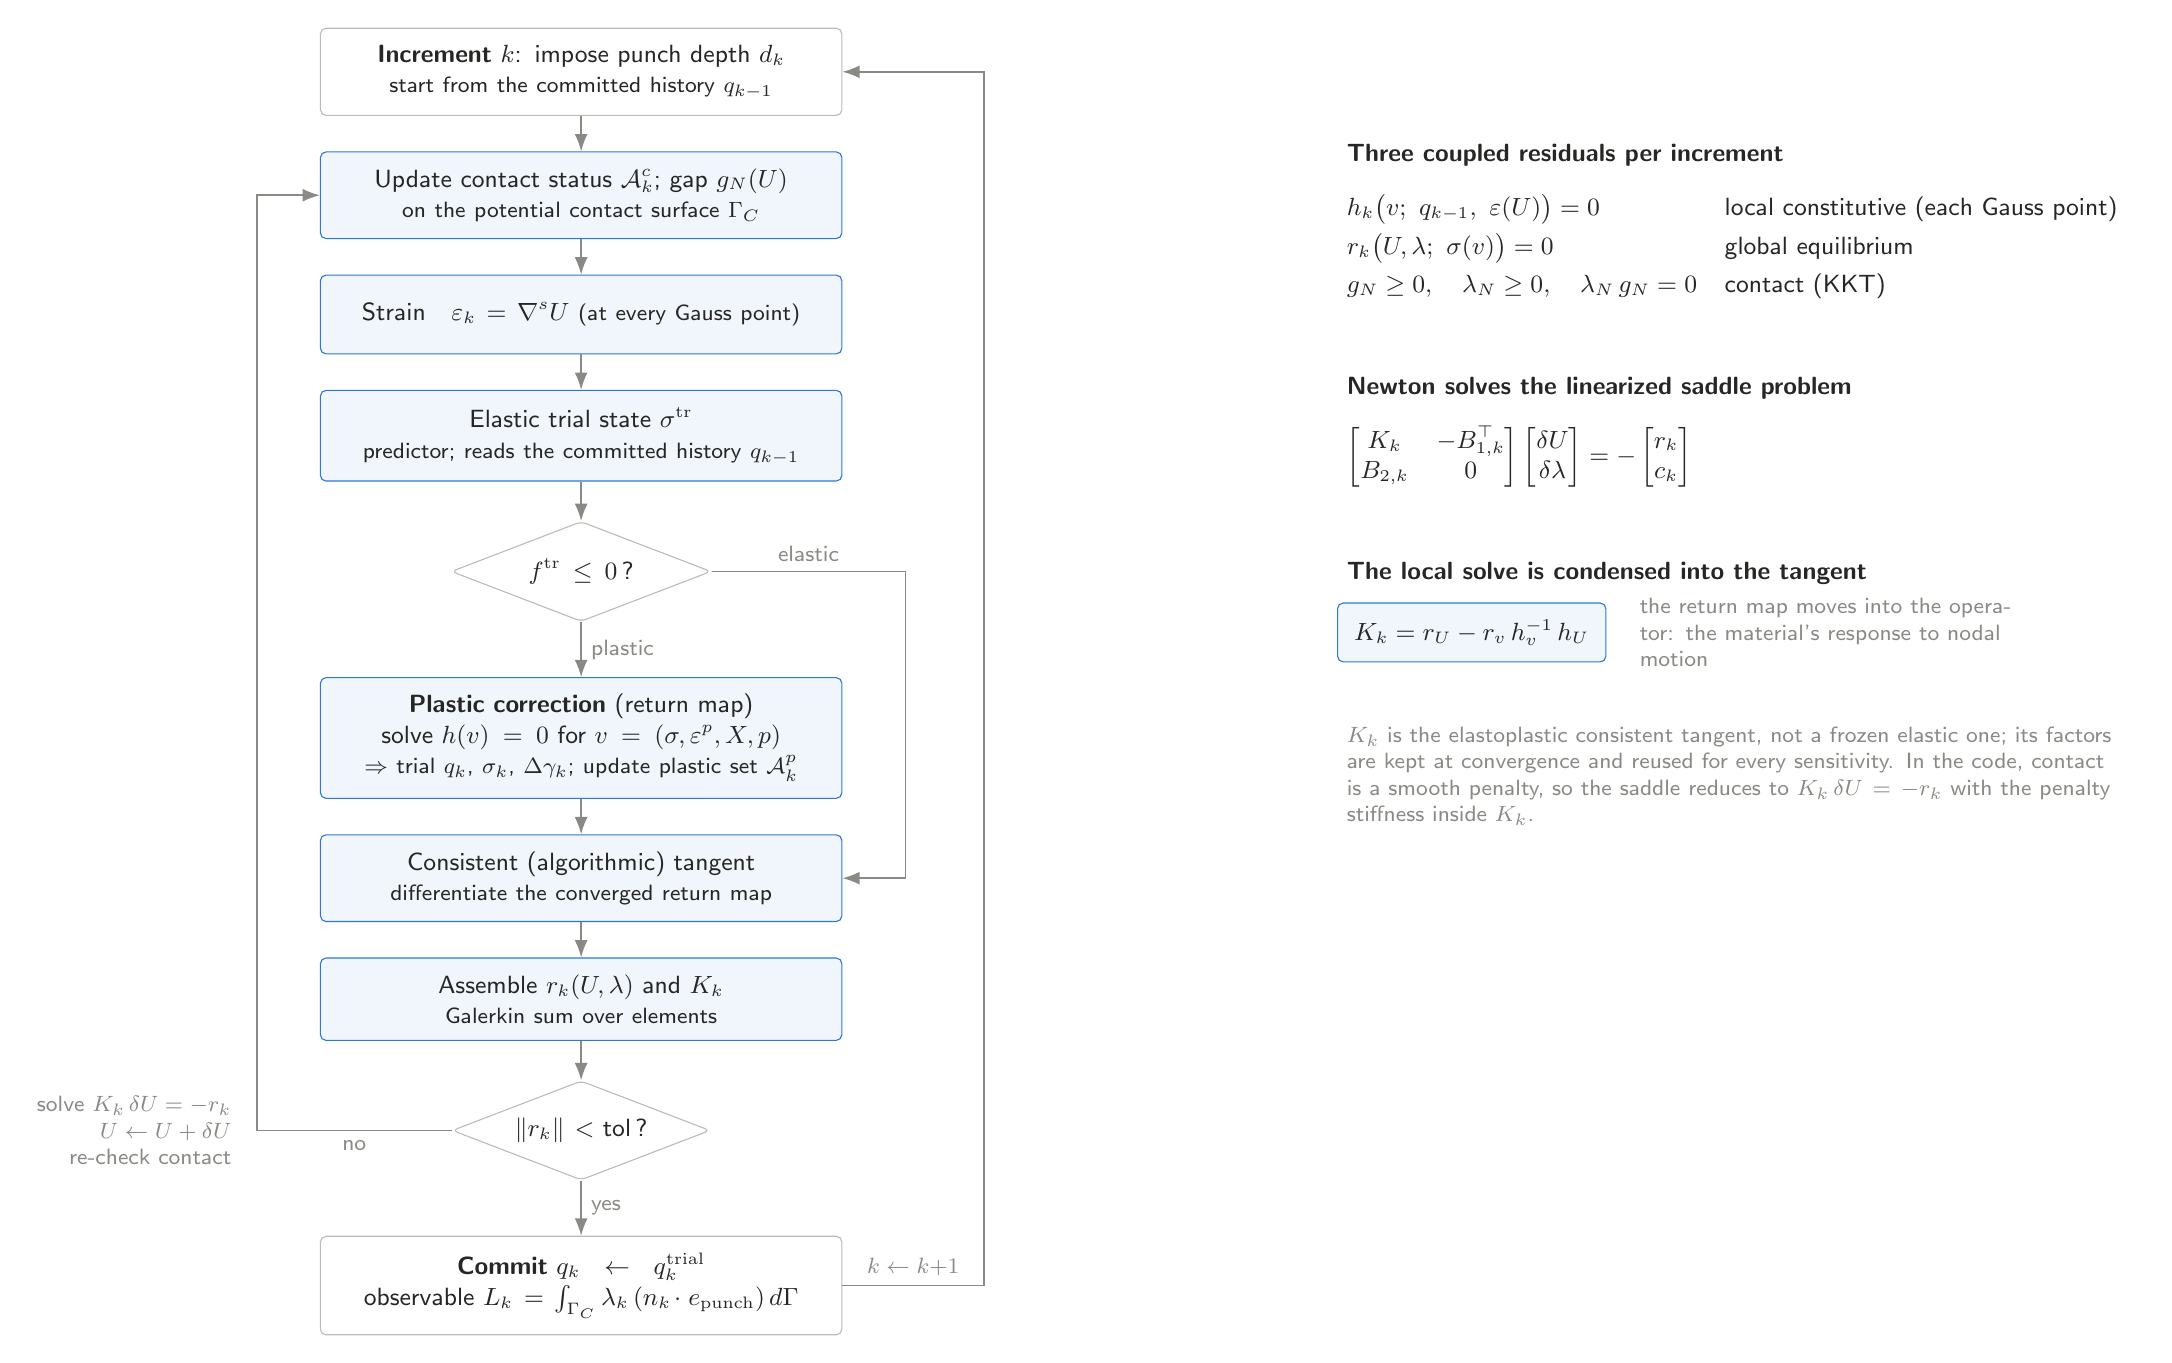
\begin{tikzpicture}[node distance=4.5mm]
% ---------------- flowchart ----------------
\node[b=62mm] (inc) {\textbf{Increment $k$}: impose punch depth $d_k$\\ {\footnotesize start from the committed history $q_{k-1}$}};
\node[a=62mm, below=of inc] (ct) {Update contact status $\mathcal A^c_k$; gap $g_N(U)$\\ {\footnotesize on the potential contact surface $\Gamma_C$}};
\node[a=62mm, below=of ct] (st) {Strain\quad $\varepsilon_k = \nabla^s U$ {\footnotesize (at every Gauss point)}};
\node[a=62mm, below=of st] (tr) {Elastic trial state $\sigma^{\rm tr}$\\ {\footnotesize predictor; reads the committed history $q_{k-1}$}};
\node[b=30mm, diamond, aspect=2.6, inner sep=1pt, below=5mm of tr, text width=22mm] (y) {$f^{\rm tr}\le 0$\,?};
\node[a=62mm, below=7mm of y] (pc) {\textbf{Plastic correction} (return map)\\ solve $h(v)=0$ for $v=(\sigma,\varepsilon^p,X,p)$\\ {\footnotesize $\Rightarrow$ trial $q_k$, $\sigma_k$, $\Delta\gamma_k$; update plastic set $\mathcal A^p_k$}};
\node[a=62mm, below=of pc] (tg) {Consistent (algorithmic) tangent\\ {\footnotesize differentiate the converged return map}};
\node[a=62mm, below=of tg] (as) {Assemble $r_k(U,\lambda)$ and $K_k$\\ {\footnotesize Galerkin sum over elements}};
\node[b=30mm, diamond, aspect=2.6, inner sep=1pt, below=5mm of as, text width=22mm] (cv) {$\|r_k\| <$ tol\,?};
\node[b=62mm, below=7mm of cv] (cm) {\textbf{Commit} $q_k \leftarrow q_k^{\rm trial}$\\ observable $L_k = \int_{\Gamma_C}\lambda_k\,(n_k\!\cdot e_{\rm punch})\,d\Gamma$};
\draw[e] (inc) -- (ct); \draw[e] (ct) -- (st); \draw[e] (st) -- (tr); \draw[e] (tr) -- (y);
\draw[e] (y) -- node[right, t]{plastic} (pc);
\coordinate (xr) at ($(inc.east)+(8mm,0)$); \coordinate (xl) at ($(inc.west)+(-8mm,0)$);
\draw[e] (y.east) -- node[above, t]{elastic} (y.east -| xr) |- (tg.east);
\draw[e] (pc) -- (tg); \draw[e] (tg) -- (as); \draw[e] (as) -- (cv);
\draw[e] (cv) -- node[right, t]{yes} (cm);
\draw[e] (cv.west) -- node[below, t]{no} (cv.west -| xl) |- (ct.west);
\node[t, align=right, anchor=east] at ($(cv.west -| xl)+(-2mm,0)$) {solve $K_k\,\delta U=-r_k$\\ $U\leftarrow U+\delta U$\\ re-check contact};
\draw[e] (cm.east) -- node[above, t]{$k\leftarrow k{+}1$} ($(cm.east -| xr)+(10mm,0)$) |- (inc.east);
% ---------------- equations ----------------
\begin{scope}[shift={(96mm,-8mm)}]
\node[anchor=north west, font=\small\bfseries] (h1) at (0,0) {Three coupled residuals per increment};
\node[anchor=north west, below=1mm of h1.south west, anchor=north west, font=\small, align=left] (eq1) {%
$\begin{aligned}
&h_k\big(v;\ q_{k-1},\ \varepsilon(U)\big)=0 &&\text{local constitutive (each Gauss point)}\\
&r_k\big(U,\lambda;\ \sigma(v)\big)=0 &&\text{global equilibrium}\\
&g_N\ge 0,\quad \lambda_N\ge 0,\quad \lambda_N\,g_N=0 &&\text{contact (KKT)}
\end{aligned}$};
\node[below=7mm of eq1.south west, anchor=north west, font=\small\bfseries] (h2) {Newton solves the linearized saddle problem};
\node[below=1mm of h2.south west, anchor=north west, font=\small] (eq2) {%
$\begin{bmatrix} K_k & -B_{1,k}^{\top}\\ B_{2,k} & 0\end{bmatrix}
\begin{bmatrix}\delta U\\ \delta\lambda\end{bmatrix}
= -\begin{bmatrix} r_k\\ c_k\end{bmatrix}$};
\node[below=7mm of eq2.south west, anchor=north west, font=\small\bfseries, text width=95mm] (h3) {The local solve is condensed into the tangent};
\node[below=1mm of h3.south west, anchor=north west, font=\small, draw=acc, fill=accbg, rounded corners=2pt, inner sep=6pt] (eq3) {%
$K_k = r_U - r_v\,h_v^{-1}\,h_U$};
\node[right=3mm of eq3, t, align=left, text width=48mm] {the return map moves into the operator: the material's response to nodal motion};
\node[below=7mm of eq3.south west, anchor=north west, t, align=left, text width=100mm] {$K_k$ is the elastoplastic consistent tangent, not a frozen elastic one; its factors are kept at convergence and reused for every sensitivity. In the code, contact is a smooth penalty, so the saddle reduces to $K_k\,\delta U = -r_k$ with the penalty stiffness inside $K_k$.};
\end{scope}
\end{tikzpicture}
\end{document}
